\chapter{O ciclo de vida do produto na I4.0}
\label{cha:ciclo-de-vida}

Este capítulo visa trazer discussões sobre o impacto do amplo compartilhamento da memória digital do produto (MDP) ao longo da cadeia de suprimentos por meio de serviços na Indústria 4.0.

% São abordadas possíveis mudanças na curva de ciclo de vida do produto e o surgimento de novos modelos de negócio baseado em dados (\textit{data-driven}).

Uma visão da MDP sobre o eixo ``Ciclo de Vida e Cadeia de Valor'' do RAMI4.0 é abordada, discutindo as atribuições dos AAS como ``tipos'' e como ``instâncias''.

Além disso, é abordada uma proposta de modelo da estrutura de dados de um AAS que compartilha as informações relacionadas ao seu estado na cadeia de suprimentos. Desta forma, é feita uma análise relacionada aos submodelos necessários para a implementação da ``Arquitetura para compartilhamento de informações do ativo'', abordada no \autoref{cha:arquitetura}.

\section{Geração de valor por meio do compartilhamento da MDP}

O modelo do RAMI4.0 descrito na \autoref{sub:rami4} apresentou o eixo ``ciclo de vida'' generalizado, cujo o objetivo é representar o ciclo de vida de um Componente I4.0 ao longo de toda a sua cadeia de valor.

O histórico completo do ciclo de vida de um determinado produto corresponde a suas informações de estados relevantes geradas ao longo de sua existência. Estas informações são acessadas via MDP, e são associadas a seu ativo tanto em sua fase ``tipo'' quanto em sua fase ``instância'' (vide \autoref{sub:rami4}). Estes dados podem ser aproveitados de forma inteligente para a geração de valor por meio de novos modelos de negócio.

A ``Arquitetura para compartilhamento de informações do ativo'' possibilita o fluxo informações entre estas duas fases do ativo (``tipo'' e ``instância''), o que traz novas possíveis formas de geração de valor. A \autoref{fig:aas-lifecycle} ilustra este cenário, onde o compartilhamento da MDP gera melhorias a partir das informações do ativo. Foram identificadas duas formas de geração de valor por meio das informações do ativo: as ``melhorias de projeto'' e as ``melhorias operacionais'', que serão discutidas na \autoref{sec:melhoria-projeto} e \autoref{sec:melhoria-operacional}.

\begin{figure}[htb!]
	\centering
	\includegraphics[width=1\textwidth]{aas-lifecycle}
	\caption{Ciclo de vida do produto.}
	\label{fig:aas-lifecycle}
\end{figure}

O fluxo de informações e geração de valor é detalhado a seguir:

\begin{enumerate}[label=(\alph*)]
	\item O projeto inicial de um produto é disponibilizado para produção em forma de um ``tipo'';
	\item Instâncias do projeto são fabricadas e disponibilizadas para venda e distribuição;
	\item Dados são coletados a partir das várias instâncias produzidas;
	\item Um alto volume de dados coletados das instâncias é análisado utilizando técnicas análise de dados e \textit{business intelligence};
	\item A partir do processamento dos dados, há criação de valor relacionada à melhoria operacional do produto (detalhada na \autoref{sec:melhoria-operacional});
	\item A partir do processamento dos dados e de outros fatores externos, há criação de valor relacionada à melhoria de projeto do produto (detalhada na \autoref{sec:melhoria-projeto});
	\item Com as melhorias de projeto, uma nova versão (tipo) é gerada, completando assim o ciclo de vida.
\end{enumerate}

A \autoref{fig:aas-lifecycle} representa o fluxo de geração de valor ao longo do ciclo de vida de um produto no contexto da Indústria 4.0. Este ciclo de vida representa o seu processo de melhoria continua por meio do compartilhamento de dados de acordo com a ``Arquitetura para compartilhamento de informações do ativo''.

Os ativos (definidos como produtos) geram, por exemplo, informações de uso e sobre manutenções realizadas, que podem ser armazenadas na MDP e assim auxiliar em melhorias no seu próprio processo de fabricação, além de ser fonte de dados para o desenvolvimento de novas versões aperfeiçoadas, gerando um novo ``tipo''.

O compartilhamento das informações insere um novo elemento na competitividade entre as empresas \cite{framling2013plm} e, por meio da MDP, este compartilhamento é possibilitado. O novos ativos inseridos neste novo ``formato'' trazem a possibilidade de exploração de seus dados e alteram, desta forma, a estrutura da indústria e a natureza da concorrência, expondo as empresas a novas oportunidades e ameaças competitivas \cite{porter2014smartproducts}.

A MDP, portanto, traz a agregação de valor ao produto como um todo por meio do compartilhamento de informações. Neste capítulo são propostas duas novas classificações quanto às formas de melhoria do produto e agregação de valor por meio da MDP: as \textbf{melhorias de projeto} (\autoref{sec:melhoria-projeto}) e as \textbf{melhorias operacionais} (\autoref{sec:melhoria-operacional}) .

A divisão em \textbf{melhorias de projeto} e \textbf{melhorias operacionais} permite segregar os tipos de informações a serem compartilhadas e assim detalhar a estrutura de dados do submodelo correspondente.

\subsection{Melhoria de projeto do produto}
\label{sec:melhoria-projeto}

%A extração de informações da MDP auxilia no desenvolvimento de novas versões com ``tipos'' aprimorados. Novos ``tipos'' aprimorados significam a melhoria de projeto do produto.

\citeonline{porter2014smartproducts} e \citeonline{porter2015smartproducts} classificaram o valor das informações dos produtos em quatro áreas: monitoramento, controle, otimização e autonomia. Por meio da análise da descrição das funcionalidades e capacidades de cada área, foi feito um mapeamento para o contexto do eixo ``ciclo de vida e cadeia de valor'' do RAMI4.0.

Os tipos de valor das informações no que diz respeito à melhoria de projeto foram então reclassificados sob o contexto do RAMI4.0. As seguintes categorias foram então definidas:

\begin{itemize}
	\item Identificação e reparo de falhas de projeto;
	\item Melhoria da interação do usuário com o produto;
	\item Geração de indicadores.
\end{itemize}

Estas categorias permitem segregar as informações de acordo com seus respectivos objetivos ao serem inseridos no projeto de um ativo. Além disso, as categoriais dão indícios de possíveis informações genéricas a serem armazenadas ao longo do ciclo de vida do produto, independente da indústria na qual ele está inserido.

A seguir são apresentadas as descrições de cada uma das categorias apresentadas:

A \textbf{``Identificação e reparo de falhas de projeto''} permite o monitoramento remoto e identificação de eventuais falhas de projeto por meio da análise de um alto volume de dados e identificação de padrões.

A  identificação de potenciais falhas se dá, por exemplo, por meio da leitura de sensores de temperatura e vibração de diversos ativos de um mesmo modelo. Valores discrepantes do esperado podem, então, serem identificados em uma amostra. Os eventuais erros estruturais de projeto deve ser reparados e lançados em um novo ``tipo'', como uma nova versão.

A \textbf{``Melhoria da interação do usuário com o produto''} se dá pela exploração e análise das informações que descrevem a maneira e padrões como o usuário interage com o ativo (produto). Desta forma, as informações podem ser utilizadas pelo fabricante para a determinação de funções que podem não ser claras para o usuários ou funções que estão sendo utilizadas de maneira incorreta.

Mudanças na ergonomia e melhorias na intuitividade das funções de operação são mudanças de projeto que elevam a experiência do usuário com o ativo e causam uma maior percepção de valor.

A melhoria de interação se dá também pela adição ou remoção de funcionalidades já existentes. A partir da análise de padrões de uso é possível determinar com o ativo é realmente utilizado e a partir disso levantar a necessidade da adição de novas funcionalidades ou até mesmo a remoção de funções pouco utilizadas.

O monitoramento das características operacionais é uma forma de evoluir o projeto por meio de sua simplificação. Desta forma, atende-se às reais necessidades do usuário e se evita produtos inflados de funcionalidades ou com funcionalidades importantes faltando.

A \textbf{``Geração de indicadores''} traz conhecimento que auxilia na tomada de decisões. Alguns indicadores dependem das circunstâncias de operação do equipamento e, portanto, variam em relação ao valor estabelecido pelo fabricante. Por meio dos indicadores, o fabricante é capaz de investigar problemas e eventualmente reprojetar o equipamento. Além disso, o próprio gestor dos equipamentos pode identificar possíveis melhorias em processos a fim de atingir determinadas metas.

Os indicadores de  volume de emissão de gases e materiais particulados e podem ser usados em auditoriais para adequação às condições legais e regulatórias do país e/ou para atender às condições de saúde e bem estar do trabalhador.

A eficiência Global do Equipamento (\textit{Overall equipment effectiveness} - OEE), o volume de emissão de gases do efeito estufa e materiais particulados e o consumo energético e eficiência energética são outros exemplos de indicadores a serem gerados e atualizados instantaneamente pelos próprios ativos.

\subsection{Melhoria operacional do produto}
\label{sec:melhoria-operacional}

% A fase ``instância'' ocorre com a produção e venda  que é feita a partir de um ``tipo'' de ativo. Informações específicas sobre produção, logística e qualidade são associadas às ``instâncias'' dos ativos.

% Nesta fase o produto está em produção, o que significa que o usuário está ativamente utilizando o produto/equipamento em sua empresa. Os dados de uso da instância podem ser compartilhados com outros parceiros da cadeia de valor.

A análise de dados da MDP traz benefícios às ``instâncias'' sem necessariamente alterar seu projeto (alterar seu tipo), ou seja, são benefícios operacionais agregados ao ativo.

A partir das classificações sobre o valor das informações dos produtos apresentadas por \citeonline{porter2014smartproducts} e \citeonline{porter2015smartproducts}, foi feito um mapeamento para as funções relacionadas às melhorias operacionais, criando uma nova classificação das informaçoes sob o contexto do eixo ``ciclo de vida e cadeia de valor'' do RAMI4.0.

Os tipos de valor das informações no que diz respeito à melhoria operacional foram então reclassificados sob o contexto do RAMI4.0. As seguintes categorias foram então definidas:

\begin{itemize}
	\item Manutenção orientada por dados;
	\item Monitoramento e rastreamento em tempo real;
	\item Integração dos membros da cadeia de suprimentos e eficiência logística.
\end{itemize}

As categorias permitem segregar as informações de acordo com seus respectivos objetivos ao serem inseridos no projeto de um ativo. Além disso, as categoriais dão indícios de possíveis informações genéricas a serem armazenadas ao longo do ciclo de vida do produto, independente da indústria na qual ele está inserido.

A seguir são apresentadas as descrições de cada uma das categorias apresentadas:

A \textbf{``Manutenção orientada por dados''} (\textit{data driven}) é uma mudança de paradigma em relação à forma tradicional como a manutenção dos ativos é realizada.

Com o histórico de leitura de sensores de cada componente do ativo, estratégias de manutenção preditivas e prescritivas podem ser adotadas pelo próprio fabricante. A manutenção orientada pelos dados de uso, comparada com a manutenção tradicional, pode reduzir a incidência de falhas e trazer benefícios econômicos. %\cite{odonovan2015maintenance}

Com a manutenção prescritiva, os dados empíricos e o histórico do ativo são utilizados para prescrever qual medida deve ser tomada, trazendo mais confiabilidade por meio de técnicas estatísticas. A contínua extração de dados de sensores do ativo e sua análise torna a ação de manutenção mais automatizada.

A manutenção dos ativos orientada por dados permite trazer a responsabilidade de manutenção dos ativos de uma planta para a instituição que melhor conhece os detalhes do funcionamento técnico do ativo, como o fabricante ou uma empresa especializada na manutenção de um determinado ativo. O uso de dados para a manutenção permite implementar um novo paradigma de detecção e correção de falhas de equipamentos industriais: a Manutenção como um Serviço (\textit{Maintenance-as-a-Service} - MaaS). %\cite{zoll2018maas}

O \textbf{``Monitoramento e rastreamento em tempo real''} é possibilitado pela leitura de coordenadas geográficas. O monitoramento e rastreamento são úteis durante o transporte entre os membros da cadeia de suprimentos. O distribuidor, por exemplo, pode ter acesso à posição exata de um ativo enquanto este estiver sob sua custódia.

As coordenadas geográficas garantem a rastreabilidade do ativo enquanto ele se desloca ao longo da cadeia de suprimentos. A demanda de rastreabilidade surge para manter um melhor controle da cadeia produtiva, assim como repassar essas informações aos consumidores.

Outra função do rastreamento é como forma de identificar possíveis parcerias ao atender a uma demanda de fabricação. Ao iniciar uma ordem de fabricação/compra, o próprio ativo pode se encarregar de selecionar quem irá fabricar, onde será entregue, qual empresa de transporte, custos, prazos, etc.

A \textbf{``Integração dos membros da cadeia de suprimentos e eficiência logística''} acontece com a melhoria da comunicação entre os elos utilizando o produto (ativo) como centro de interação.

A comunicação passa ser centralizada e não mais depender pelo contato direto entre as partes. Isso simplifica também a logística reversa, como no caso de reciclagem, acionamento da garantia, \textit{recalls} e outros.

Outro ponto de melhor integração com a utilização do produto como centro das interações é com relação à documentação. O submodelo de documentação conterá todos os documentos digitais referentes ao ativo. Desta forma, manuais, notas fiscais, certificados de manutenção e outros documentos podem ser escritos, lidos e atualizados pelos parceiros da CS mediante autenticação.

O compartilhamento de documentos digitais permite uma maior interação com as partes e garante que cada membro terá sempre a versão mais atualizada de um determinado documento, favorecendo assim sua gestão, reduzindo o uso do papel e tornando os ambientes de trabalho mais seguros, ágeis e organizados.

Os documentos representam uma conexão entre os membros da CS, portanto, comunicados, formulários de troca, documentos para acionamento de garantia, \textit{recalls} e quaisquer outras operações que envolvam a logística reversa podem ser solicitados pela própria MDP.

\section{Submodelos e propriedades dos componentes}

Nesta seção são apresentadas propostas de submodelos e propriedades necessárias para a integração dos ativos na cadeia de suprimentos.

Os submodelos dos componentes da ``Arquitetura para compartilhamento de informações do ativo'' devem ser padronizados e detalhados a fim de se garantir a interoperabilidade entre os sistemas.

São apresentados os submodelos essenciais do ``AAS-Repositório'' e ``AAS-Servidor''. A fim de simplificação, o AAS-Repositório será mencionado como ``repositório'' e o AAS-Servidor como ``produto''.

\subsection{Submodelos do repositório}

O repositório armazena as descrições dos serviços definidos pelos contratos de cada \textit{Web Service}, que são publicados por diversos ativos no mundo conectado da Indústria 4.0.

Os dados dos contratos contidos no repositório devem ser padronizados para garantir uma interpretação consistente por parte das aplicações, que consomem os serviços. Para isso, os submodelos do repositório devem ser estabelecidos a fim de se criar moldes de metamodelos sobre os quais os dados devem ser estruturados.

\citeonline{bader2019aas} estabelece padrões de metamodelos para a implementação de submodelos no AAS, porém não aborda um possível repositório de serviços e o armazenamento de dados de serviços.

A proposta de estruturação dos dados do repositório é dividida em três submodelos: ``serviço'', ``produto'' e ``contrato''. As Tabelas \ref{tab:repositorio-submodelo-servico}, \ref{tab:repositorio-submodelo-produto} e \ref{tab:repositorio-submodelo-contrato} detalham as propriedades de cada um dos submodelos.

\begin{table}[htb]
	\centering
	\caption{Submodelo ``serviço'' do repositório.}
	\begin{tabular}{p{2.5cm}p{1.5cm}p{9.5cm}}
		\hline
		\textbf{Propriedade}
		 & \textbf{Tipo}
		 & \textbf{Descrição}                                                                                                                                                                                                                                                                                                                                                                                                                                         \\

		\hline
		\textit{id}
		 & \textit{String}
		 & Número do serviço para a sua identificação única dentre todos os repositórios. O ID do serviço deve ser derivado do próprio ID do AAS-Servidor correspondente como um \textit{namespace} (E.g., ID\_SERVIDOR. ID\_SERVIÇO\_001).                                                                                                                                                                                                                           \\

		\hline
		\textit{description}
		 & \textit{String}
		 & Descrição textual sobre as funcionalidades do \textit{Web Service}. Está é uma descrição textual, pois a descrição completa é estabelecida no formato padronizado dp contrato do \textit{web service}.                                                                                                                                                                                                                                                     \\

		\hline
		\textit{reputation}
		 & \textit{Integer}
		 & A métrica de reputação fornece indicadores sobre a qualidade do serviço prestado por um determinado AAS. O tempo médio de resposta do serviço baseado no tempo de resposta observado por diversas requisições executadas e a disponibilidade do AAS quando solicitado são índices que compõem o índice de reputação. Um índice para serviços cuja qualidade é subjetiva pode ser criado baseado em avaliações de AAS Clientes que já consumiram o serviço. \\

		\hline
		\textit{product\_id}
		 & \textit{String}
		 & Referência ao produto o qual fornece este determinado serviço.                                                                                                                                                                                                                                                                                                                                                                                             \\

		\hline
	\end{tabular}
	\label{tab:repositorio-submodelo-servico}
\end{table}

\begin{table}[htb]
	\centering
	\caption{Submodelo ``produto'' do repositório.}
	\begin{tabular}{p{3cm}p{2cm}p{9cm}}
		\hline
		\textbf{Propriedade}
		 & \textbf{Tipo}
		 & \textbf{Descrição}                                                                                                                                                                                                                                                                                                                                               \\

		\hline
		\textit{id}
		 & \textit{String}
		 & Tem a função de distinguir exclusivamente os AAS provedores de serviços e todos seus elementos \cite{adolphs2016structure} no mundo conectado da I4.0. Alguns tipos possíveis de identificadores são \cite{bader2019aas}: IRDI, IRI e UUID. O ID do AAS servidor permite que o consumidor dos serviços possa localizar e invocar diretamente o serviço ofertado. \\

		\hline
		\textit{description}
		 & \textit{String}
		 & Breve descrição sobre o AAS Servidor como nome, modelo e companhia fabricante do ativo.                                                                                                                                                                                                                                                                          \\
		\\

		\hline
		\textit{reputation}
		 & \textit{Integer}
		 & Corresponde à média dos índices de reputação de todos os serviços daquele produto                                                                                                                                                                                                                                                                                \\

		\hline
	\end{tabular}
	\label{tab:repositorio-submodelo-produto}
\end{table}

\begin{table}[htb]
	\centering
	\caption{Submodelo ``contrato'' do repositório.}
	\begin{tabular}{p{3.5cm}p{1.5cm}p{9cm}}
		\hline
		\textbf{Propriedade}
		 & \textbf{Tipo}
		 & \textbf{Descrição}                                                                                                                                                                                                                                                                 \\

		\hline
		\textit{id}
		 & \textit{String}
		 & UUID do contrato.                                                                                                                                                                                                                                                                  \\


		\hline
		\textit{contract\_definition}
		 & \textit{String}
		 & Arquivo de definição do contrato, que é a documentação da API. Este documento descreve o comportamento da API, o que inclui as URLs dos \textit{endpoints} (rotas), os métodos de cada rota, argumentos e exemplos de chamadas (\textit{requests}) com suas respectivas respostas. \\

		\hline
		\textit{version}
		 & \textit{Integer}
		 & Versão do contrato.                                                                                                                                                                                                                                                                \\

		\hline
		\textit{insertion\_time}
		 & \textit{Datetime}
		 & \textit{Timestamp} do momento de registro desta versão específica do contrato no repositório.                                                                                                                                                                                      \\

		\hline
		\textit{service\_id}
		 & \textit{String}
		 & Referência ao ID do serviço associado a este contrato.                                                                                                                                                                                                                             \\


		\hline
	\end{tabular}
	\label{tab:repositorio-submodelo-contrato}
\end{table}

A \autoref{fig:submodelos-repositorio} mostra a interrelação entre os submodelos apresentados nas Tabelas \ref{tab:repositorio-submodelo-servico}, \ref{tab:repositorio-submodelo-produto} e \ref{tab:repositorio-submodelo-contrato}.

\begin{figure}[htb!]
	\centering
	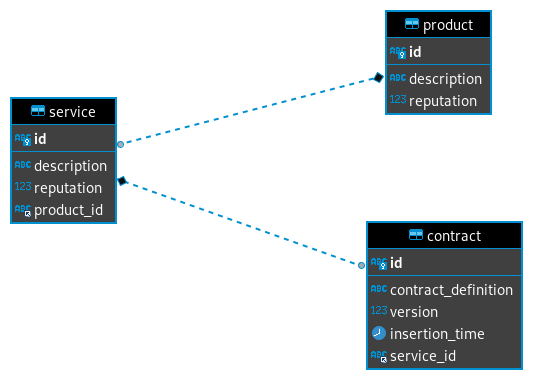
\includegraphics[width=1\textwidth]{submodelos-repositorio}
	\caption{Submodelos do repositório e suas interrelações.}
	\label{fig:submodelos-repositorio}
\end{figure}

O submodelo ``serviço'' possui a chave estrangeira \textit{product\_id} com referência à chave primária \textit{id} do submodelo ``produto''. Os submodelos ``serviço'' e ``produto'' mantêm uma relação de n para 1, uma vez que um produto pode conter diversos serviços, mas um serviço pertence a um e somente um produto.

O submodelo ``contrato'' possui a chave estrangeira \textit{service\_id} com referência à chave primária \textit{id} do submodelo ``serviço''. Os submodelos ``serviço'' e ``contrato'' mantêm uma relação de 1 para n, uma vez que um serviço pode conter diversos contratos em diferentes versões e os contratos pertencem a exclusivamente um serviço.

Os três submodelos apresentados e suas propriedades não são exaustivas. Entende-se que estes são submodelos básicos para permitir o armazenamento, identificação, e compartilhamento de descrições de serviços. Mais submodelos e novas definições surgirão a fim de se adicionar novas funcionalidades ao repositório.

% O cliente consumidor (AAS-Cliente) na operação de busca fará uma requisição ao repositório ou a uma lista de repositórios e receberá via API a lista de serviços providenciada por meio dos contratos.

O produto (AAS-Servidor) é o responsável pela geração e atualização dos dados referentes a seus serviços no AAS-Repositório. Dados relacionados ao índice de reputação, entretanto, devem ser gerados pelo próprio repositório para garantir a integridade dos índices.

A inserção e atualização de um registro no repositório deve acontecer sempre que um produto é instalado ou atualizado, o que acarreta uma nova operação de publicação, gerando assim uma nova versão do contrato.

%\section{Submodelos e propriedades para a integração da cadeia de valor}

\section{Submodelos do produto}

O produto no contexto da ``Arquitetura para compartilhamento de informações do ativo'' o Componente I4.0 é a fonte e o servidor de informações para os diversos membros ao longo da cadeia de suprimentos. O acesso a estas informações permite a colaboração entre os membros e assim abre oportunidades para uma tomada de decisões coordenada a fim de remover as ineficiências inerentes da cadeia de suprimentos.

É necessária uma definição dos submodelos do produto a fim de se identificar os tipos de informações genéricas a ser compartilhadas e com quais membros compartilhar. Além disso, a definição destes submodelos contribui com o refinamento das especificações do AAS no contexto da Indústria 4.0.

\citeonline{torres2014information} faz uma análise da literatura bibliográfica e analisa o impacto do compartilhamento de informações em cadeias de suprimentos. Além disso, é feita uma classificação dos trabalhos, dentre elas a classificação quanto ao tipo de informação a ser compartilhada, apresentando também a descrição de informações comumente mencionadas nos trabalhos.

Os tipos de informações identificados na análise bibliográfica de \citeonline{torres2014information} serão incorporados a seus respectivos submodelos no AAS-Servidor para que possam ser compartilhadas por meio da MDP. Os submodelos a serem criados com base nos tipos de informações identificados na análise bibliográfica são: ``Produto'', ``Processo'', ``Recurso'', ``Inventário'', ``Pedido'' e ``Planejamento''.

%Além disso, os submodelos ``Dados técnicos'', ``Dados Operacionais'' e ``Documentação'' segundo \citeonline{bader2020submodel} também serão incorporados ao AAS do produto. Como ``Produto'' e ``Dados técnicos'' remetem a dados semelhantes, estes submodelos serão fundidos em um.

%Portanto, são detalhados os seguintes submodelos referentes ao AAS-Produto: ``Processo'', ``Recursos'', ``Inventário'', ``Pedido'', ``Planejamento'', ``Dados técnicos'', ``Dados Operacionais'' e ``Documentação'' (Tabelas \ref{tab:produto-submodelo-processo}, \ref{tab:produto-submodelo-recursos}, \ref{tab:produto-submodelo-inventario}, \ref{tab:produto-submodelo-pedido}, \ref{tab:produto-submodelo-planejamento}).

O objetivo de se especificar os submodelos de um AAS é o estabelecimento de um formato padrão de estrutura de dados, criando uma interface pela qual desenvolvedores, fabricantes e editores de documentação técnica possam se basear na hora de descrever o AAS de seus próprios produtos.

\subsection{Submodelo ``produto''}

O AAS-Servidor (AAS do produto) deverá conter um submodelo que representa as informações do produto em si, o que inclui sua ficha com dados técnicos e dados operacionais.

As informações do produto descrevem as características do produto fabricado na cadeia de suprimentos e seu processo de produção.

A \autoref{tab:produto-submodelo-produto} detalha o submodelo ``produto'' com suas respectivas propriedades.

\begin{table}[htb]
	\centering
	\caption{Submodelo ``produto''.}
	\begin{tabular}{p{3.5cm}p{1.5cm}p{9cm}}
		\hline
		\textbf{Propriedade}
		 & \textbf{Tipo}
		 & \textbf{Descrição}                                                                                                                                                                                                                  \\

		\hline
		Estrutura do produto
		 & \makecell{List\\{[String]}}
		 & Lista de materiais (\textit{Bill of Materials} - BOM) com os materiais e quantias necessárias para a fabricação do respectivo produto. Organizar a produção de diversos produtos na fábrica e garante a padronização dos processos. \\

		\hline
		Ficha técnica
		 & \makecell{List\\{[String]}}
		 & Informações gerais sobre o produto como seu modelo, seu número de série, fabricante, etc.                                                                                                                                           \\

		\hline
		Dados operacionais
		 & \makecell{List\\{[Float]}}
		 & Dados relacionados ao funcionamento do produto, como o histório de leitura de sensores e padrões de uso.                                                                                                                            \\

		\hline
		Documentação
		 & \makecell{List\\{[Blob]}}
		 & Arquivos relacionado ao produto como comprovantes e manuais devidamente versionados.                                                                                                                                                \\

		\hline
	\end{tabular}
	\label{tab:produto-submodelo-produto}
\end{table}

\subsection{Submodelo ``processo''}

O submodelo ``processo'' descreve informações relacionadas a processos de negócio que adicionam valor ao produto a fim de satisfazer as demandas do cliente, isto é, as etapas de pedido, produção e envio.

A etapa de pedido começa quando um comprador que faz um pedido ao fornecedor e termina quando o fornecedor aceita o pedido. A etapa de produção ocorre com a transformação dos materiais de entrada em um produto de maior valor. A etapa de envio entrega as mercadorias do fornecedor ao comprador. Diferentes tipos de informações estão relacionados a cada uma destas etapas.

A \autoref{tab:produto-submodelo-processo} detalha o submodelo ``processo'' com suas respectivas propriedades.

\begin{table}[htb]
	\centering
	\caption{Submodelo ``processo''.}
	\begin{tabular}{p{3.5cm}p{1.5cm}p{9cm}}
		\hline
		\textbf{Propriedade}
		 & \textbf{Tipo}
		 & \textbf{Descrição}                                                                                                                                                                                                                                                                        \\

		\hline
		\textit{Lead time} de manufatura
		 & \textit{Float}
		 & O \textit{lead time} de manufatura (ou lead time de fabricação) é o período de tempo necessário para fabricar um item, incluindo tempo de preparação do pedido, tempo de fila, tempo de preparação, tempo de execução, tempo de movimentação, tempo de inspeção e tempo de armazenamento. \\

		\hline
		Variância do \textit{lead time} de produção
		 & \textit{Float}
		 & Medida de dispersão mostrando o quão distante cada valor do conjunto de valores de \textit{lead time} de produção está do valor médio.                                                                                                                                                    \\

		\hline
		\textit{Lead time} de entrega
		 & \textit{Float}
		 & Tempo de entrega de um determinado produto. Um valor mais curto garante que os clientes recebam os produtos rapidamente.                                                                                                                                                                  \\

		\hline
		Custo do processo de fabricação
		 & \textit{Double}
		 & Custo total do processo de fabricação. O compartilhamento dos custos do processo é necessário no planejamento integrado da cadeia de suprimentos.                                                                                                                                         \\

		\hline
		Qualidade do processo de fabricação
		 & \textit{Float}
		 & Agregação de um conjunto de dados estatísticos relacionados à qualidade do processo produtivo de um fabricante. O compartilhamento de informações relacionadas à qualidade é importante para o estabelecimento de confiabilidade no processo de fabricação do fabricante.                 \\

		\hline
		Informações da remessa
		 & \makecell{List\\{[String]}}
		 & Informações sobre a remessa na qual o produto foi entregue, como a quantidade de produtos enviada a um cliente. O fornecedor usa essas informações para aproximar a demanda de modo a reduzir o ``efeito chicote''.                                                                       \\

		\hline
		Custo de preparação
		 & \textit{Float}
		 & O custo de preparação da produção influencia no custo do lote de pedidos. A medida que o tamanho do lote de pedidos aumenta, reduz-se o custo total da demanda uma vez que reduz o custo de preparação total.                                                                             \\

		\hline
	\end{tabular}
	\label{tab:produto-submodelo-processo}
\end{table}

\subsection{Submodelo ``recurso''}

O submodelo ``recurso'' agrega informações relacionadas aos recursos necessários para a produção de um determinado produto.

O compartilhamento de informações de capacidade de cada um dos recursos na cadeia de suprimentos é útil para o planejamento integrado e a seleção de fornecedores. Desta forma, é possível identificar os fornecedores que estão dispoiníveis para receber uma determinada demanda a partir do produto.

A \autoref{tab:produto-submodelo-recurso} detalha o submodelo ``recurso'' com suas respectivas propriedades.

\begin{table}[htb]
	\centering
	\caption{Submodelo ``recurso''.}
	\begin{tabular}{p{3.5cm}p{1.5cm}p{9cm}}
		\hline
		\textbf{Propriedade}
		 & \textbf{Tipo}
		 & \textbf{Descrição}                                                                                                                                                                                                                                                                                                                                                      \\

		\hline
		Capacidade
		 & \textit{Float}
		 & Quantidade máxima de produtos ou processos que uma unidade de recurso (por exemplo uma máquina, um fornecedor ou uma estação) pode suportar. Cada unidade de recurso pode ser capaz de realizar diferentes operações e produzir diferentes tipos de produtos ou componentes. A capacidade de uma unidade de recurso indica a capacidade de satisfazer a demanda futura. \\

		\hline
		Variância da Capacidade
		 & \textit{String}
		 & Medida de dispersão da capacidade máxima do recurso, indicando sua variação em relação ao valor médio.                                                                                                                                                                                                                                                                  \\

		\hline
	\end{tabular}
	\label{tab:produto-submodelo-recurso}
\end{table}

\subsection{Submodelo ``inventário''}

O submodelo ``inventário'' agrega informações realcionadas ao gerenciamento do inventário daquele determinado produto.  O objetivo destas informações é a visibilidade do inventário de forma que seja possível ter um determinado produto para venda no momento certo e ao mesmo tempo reduzir custos relativos a estoque.

Informações relacionadas a inventário auxiliam na tomada de decisões sobre quando realizar pedidos ao fabricante, a quantidade de materiais a serem solicitados e onde armazenar.

A \autoref{tab:produto-submodelo-inventario} detalha o submodelo ``inventário'' com suas respectivas propriedades.

\begin{table}[htb]
	\centering
	\caption{Submodelo ``inventário''.}
	\begin{tabular}{p{3.5cm}p{1.5cm}p{9cm}}
		\hline
		\textbf{Propriedade}
		 & \textbf{Tipo}
		 & \textbf{Descrição}                                                                                                                                           \\

		\hline
		Nível do inventário
		 & \textit{Integer}
		 & Quantidade atual de itens de um determinado produto em estoque.                                                                                              \\

		\hline
		Custo de retenção
		 & \textit{Double}
		 & Custo necessário decorrente da manutenção em estoque um determinado produto.                                                                                 \\

		\hline
		Custos cumulativos
		 & \textit{Double}
		 & Custo cumulativo total decorrente da manutenção de itens excedentes de um produto em estoque por um determinado período de tempo.                            \\

		\hline
		Nível de serviço
		 & \textit{Float}
		 & Probabilidade esperada de não ocorrer falta de estoque durante o próximo ciclo de reabastecimento e, portanto, a probabilidade de não perder vendas futuras. \\

		\hline
	\end{tabular}
	\label{tab:produto-submodelo-inventario}
\end{table}

\subsection{Submodelo ``pedido''}

Um pedido contém informações sobre a demanda do cliente final para os fornecedores anteriores. As informações do pedido incluem a quantidade de itens no pedido, data de vencimento e tamanho do lote.

Compartilhar informações de quantidade de pedido entre as partes da cadeia de suprimentos ajuda na visibilidade do estado atual de um pedido por todos os membros.

A \autoref{tab:produto-submodelo-pedido} detalha o submodelo ``pedido'' com suas respectivas propriedades.

\begin{table}[htb]
	\centering
	\caption{Submodelo ``pedido''.}
	\begin{tabular}{p{3.5cm}p{1.5cm}p{9cm}}
		\hline
		\textbf{Propriedade}
		 & \textbf{Tipo}
		 & \textbf{Descrição}                                                                                             \\

		\hline
		Demanda
		 & \textit{Integer}
		 & Quantidade de lotes de um produto solicitados em forma de um ``pedido''. Representa uma demanda de fabricação. \\

		\hline
		Variância da demanda
		 & \textit{Float}
		 & Medida de dispersão da quantidade de pedidos em uma demanda com relação ao valor médio.                        \\

		\hline
		Tamanho do lote
		 & \textit{Float}
		 & Quantidade de itens do produto contida em uma demanda.                                                         \\

		\hline
		Data de vencimento
		 & \textit{Datetime}
		 & Prazo limite para a entrega de uma determinada demanda.                                                        \\

		\hline
	\end{tabular}
	\label{tab:produto-submodelo-pedido}
\end{table}

\subsection{Submodelo ``planejamento''}

As informações de ``planejamento'' englobam as informações relacionadas à previsão de demanda e programação de pedidos feita por cada um dos membros da cadeia de suprimentos.

A \autoref{tab:produto-submodelo-planejamento} detalha o submodelo ``planejamento'' com suas respectivas propriedades.





\begin{table}[htb]
	\centering
	\caption{Submodelo ``planejamento''.}
	\begin{tabular}{p{3.5cm}p{1.5cm}p{9cm}}
		\hline
		\textbf{Propriedade}
		 & \textbf{Tipo}
		 & \textbf{Descrição}                                                                                                                                                                                                                     \\

		\hline
		Previsão de demanda
		 & \textit{Float}
		 & Previsão de demanda de um determinado produto feita por um elo da cadeia de suprimentos. Com as previsões de demanda compartilhadas, é possível estabelecer uma alocação ótima dos recursos de produção entre os membros como um todo. \\

		\hline
		Modelo de previsão
		 & \textit{---}
		 & Modelo utilizado para o cálculo da previsão de demanda.                                                                                                                                                                                \\


		\hline
		Programação da produção
		 & \textit{Float}
		 & Alocação de recursos para a produção de um determinado produto para um período de tempo no futuro.                                                                                                                                     \\


		\hline
		Horizonte de planejamento
		 & \textit{Datetime}
		 & Período de tempo correspondente à programação da produção.                                                                                                                                                                             \\

		\hline
	\end{tabular}
	\label{tab:produto-submodelo-planejamento}
\end{table}
